\documentclass[12pt]{article}
 
\usepackage[utf8]{inputenc}
\documentclass[12pt]{article}

\usepackage{hyperref}
\usepackage[spanish]{babel}
\usepackage{float}
\usepackage{listings}

\usepackage[colorinlistoftodos]{todonotes}
\setlength {\marginparwidth }{2cm}


\title{%
Práctica 1. Información bursátil de una compañía cotizada en el IBEX35\\
\large Tipología y Ciclo de Vida de los Datos}
\author{Daniel Díaz Fernández}
\date{8 de noviembre de 2020}

\begin{document}
\maketitle

\begin{figure}[H]
    \centering
    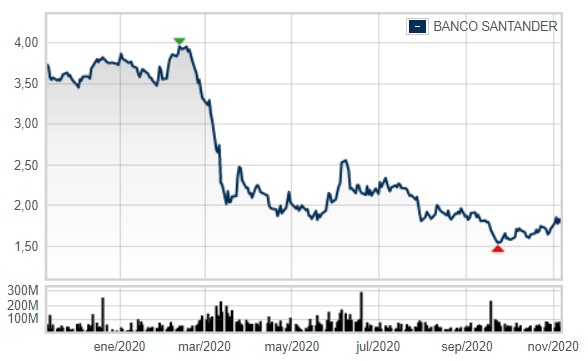
\includegraphics[width=1\columnwidth]{bolsa.jpg}
    \caption{Fluctuación anual de la acción del Banco Santander} 
    \label{flowchart}
\end{figure}

\clearpage
\section*{Contexto de los datos}
En el ámbito financiero, una 'bolsa' es un lugar en el que cotizan los productos financieros ligados, es decir, en el que se comercializa con acciones, ETF, futuros, etc. Cada día se publica la información de apertura y cierre de cualquier producto financiero. En el caso de España, la bolsa de referencia es la bolsa española de Madrid, la cual abre todos los días a las 9:00 y cierra a las 17:30 de la tarde. En ese transcurso horario, los productos financieros tienen una volatilidad de mercado que se refleja en franjas de 5 minutos, dicho de otra manera, cada 5 minutos se publica su valor monetario.\\

La información que se ha recolectado proviene de las empresas que conforman el índice IBEX35, que es el índice de referencia en nuestro país. Ese índice corresponde a las 35 empresas con mayor capitalización bursátil. Además, esta información es accesible a cualquier ciudadano sea o no de España.\\

Delante de la crisis de la COVID-19 que estamos viviendo, me he interesado por este sector financiero ya que tiene una trascendencia muy importante en la situación actual. Aunque muchas veces no lo creamos, el IBEX35 puede tener una relación directa con nuestras vidas, pues como estamos viendo, el hundimiento de algunas empresas en las bolsas nacionales e internacionales tienen que ver con las relaciones contractuales que tenemos los ciudadanos con dichas empresas. Un ejemplo directo son los bancos, que tras haber perdido gran parte de su capitalización a los meses previos a esta crisis, se han visto obligados a fusionarse, elevar las comisiones, empeorar las condiciones a sus clientes (en beneficio de ellos) e incluso, reducir costes y personal para sobrevivir a esta pandemia. Por este motivo creo que es muy importante estar lo más actualizado posible a la economía que tan lejana vemos a veces.


\section*{Descripción y contenido del dataset}
A pesar de haber cuatro bolsas en España (Madrid, Barcelona, Bilbao y Valencia), se ha escogido la bolsa de Madrid porque es la bolsa de referencia para el IBEX35 y la que más volumen de acciones mueve a diario. 

La página \url{www.bolsamadrid.es} ha sido la escogida para la obtención de los datos, que es el sitio web oficial de la bolsa de Madrid. Hay muchas otras fuentes (no oficiales) para acceder a los datos, aunque muchas de ellas son de pago o tienen un número limitado de peticiones por IP. 

El dataset contiene información financiera sobre cualquier empresa del IBEX35, las cuales corresponden al mercado financiero español. La información que se extrae de cada compañía corresponde a los siguientes atributos:
\begin{itemize}
	\item \textbf{Nombre de la empresa}: Nombre completo de la empresa, incluyendo su tipología empresarial.
	\item \textbf{Ticker}: Ticket o símbolo informativo con el que cotizan las acciones de dicha empresa en un determinado mercado bursátil. Son unas siglas alfanuméricas.
	\item \textbf{Mercado}: Tipo de mercado en el que cotizan las acciones. En nuestro caso, corresponde al mercado continuo. Que es el mercado predominante en las acciones del IBEX35. En este mercado se conecta a los operadores financieros con las bolsas españolas de forma que permite ejecutar órdenes de compra y venta de acciones de cualquier valor cotizado y desde cualquier lugar y dispositivo conectado a las bolsas.
	\item \textbf{Capital Admitido}: Corresponde a la capitalización bursátil de la empresa. Este valor viene dado por la multiplicación del número de acciones de la empresa y el valor de cada una de estas acciones. 
	\item \textbf{Información histórica}: Corresponde a las cotizaciones de los últimos días, meses o años de las acciones de la empresa. Se han recolectado todos los atributos que proporciona la web, ya que la información histórica de una empresa es muy relevante si quisiéramos realizar análisis técnicos para determinar el valor a futuro de una acción. Los atributos recolectados son los siguientes:
	\begin{enumerate}
	\item \textbf{Fecha}: Día laborable en el que cotizan las acciones.
	\item \textbf{Cierre}: Precio de cierre al final del día. Es el precio que tiene la acción justo en el momento que cierra la bolsa (17:30h en el caso de las bolsas españolas).
	\item \textbf{Referencia}: 
	\item \textbf{Volumen}: Es la cantidad de acciones que se cruzan en el día.
	\item \textbf{Efectivo}: Es la cantidad de dinero en efectivo que se cruza durante el día.
	\item \textbf{Último}: Último precio informado del día. En el caso de que el día haya pasado, el último precio y el de cierre son iguales. En caso en que el día esté en trascurso, el último precio y el de cierre probablemente serán distintos.
	\item \textbf{Máximo}: Precio máximos que ha alcanzado la acción en el día.
	\item \textbf{Mínimo}: Precio mínimo que ha alcanzado la acción en el día.
	\item \textbf{Medio}: Precio medio que ha tenido la acción en el trascurso del día.
	\end{enumerate}
	
	Es necesario aclarar que el nombre de la empresa, ticker y mercado suelen ser continuos, a no ser que la empresa tome una decisión corporativa y decida cambiar alguno de los tres atributos, en nuestro caso no ha sido así de ninguna de las treinta y cinco empresas del IBEX35 (incluidas las empresas de La Caixa y Bankia que aún no han ejecutado la fusión oficialmente). La información que sí varía cada día son la capitalización bursátil y la información histórica. La información histórica extraída representa las cotizaciones de los últimos treinta días. Se ha considerado rango de tiempo suficiente, pues para hacer \textit{trading} es un rango de tiempo más que amplio para estudiar el valor en cuestión.
\end{itemize}

\section*{Solución planteada}
Para la obtención de los datos de esta práctica se han implementado los conocimientos explicados en los temas 'Web Scraping' y 'El lenguaje Python' de la asignatura Tipología y Ciclo de Vida de los Datos, impartida en la Universitat Oberta de Catalunya.
La solución se detalla en los siguientes pasos:
\begin{itemize}
	\item \textbf{Extraer URL de la compañia deseada}. Realizamos una búsqueda de la empresa que queremos investigar a partir del buscador que posee la página, con el fin que nos devuelva el subdominio o página relativa al dominio (con los atributos necesarios en la petición) para acceder al recurso HTML que estudiaremos. En este caso, necesitamos la página que visualice una única compañía, su 'ISIN' (International Securities Identification Number, en inglés o Número de Identificación de Seguridad Internacional, en castellano) y el 'ClvEmis' (Customer Lifetime Value o Valor del Tiempo de vida del Consumidor)
	
	\item \textbf{Realizar la petición del recurso HTML}. Se realiza la petición al servidor y si éste responde con un código 200 (código de respuesta correcta), nos devolverá la página HTML para su visualización en un explorador web.
	\item \textbf{Analizar los tags del recurso HTML}. Mediante Python y las librerías de BeautifulSoup y lxml, se captura el recurso y se realizan técnicas de Web Scraping para extraer la información de cada tag HTML y almacenarlos en memoria.
	\item \textbf{Guardar datos en CSV (Comma-separated value)}. Una vez están cargados los valores en memoria se procede a almacenarlos en dos archivos csv para tenerlos permanentemente. Uno pertenece a la información de la compañía y el otro a los datos históricos de ésta.
\end{itemize}

\section*{Agradecimientos}
El propietario de la información recogida en esta práctica corresponde al Grupo BME (Bolsas y Mercados Españoles), empresa privada que se encarga de operar en todos los mercados de valores y sistemas financieros en España.
Los datos han sido recogidos a través de peticiones HTML y procesadas con Python y sus librerías para realizar Web Scraping.

\section*{Inspiración}
Este conjuntos de datos es de gran interés para múltiples ámbitos de nuestra sociedad. Como bien sabemos, la economía está presente en todos y cada uno de los sectores: salud, educación, investigación... Dominar o al menos, tener unas nociones básicas de finanzas, además de intentar estar al día de las últimas noticias puede ser muy relevante a lo largo de nuestra vida como ciudadano.\\

Considero que es muy importante saber qué se hacen con el dinero del contribuyente, ya que muchas veces porciones de empresas privadas son potestad del gobierno y por ende, un declive o malversación de dinero en una empresa privada puntera en la economía de un país suele tener implicaciones en ese gobierno. \\

Cabe destacar que muchas de las empresas privadas de nuestro país tienen sectores estratégicos muy importantes en nuestro día a día y que la pérdida de calidad en uno de ellos, tiene relación directa en otros ámbitos. 

\section*{Licencia}
La licencia seleccionada para este conjunto de datos ha sido \textbf{No-Comercial License}. Los motivos por los que se ha escogido esta licencia refieren a las cláusulas estipuladas en el Grupo BME.
\begin{itemize}
	\item \textbf{Datos accesibles a cualquiera}. Los datos son accesibles desde cualquier dispositivo, en cualquier momento y lugar.
	\item \textbf{No se permite su fin comercial}. Según el BME: 'Para llevar a cabo cualquier otro uso con fines comerciales y/o que implique la redifusión a terceros de dicha información es necesario contar con la autorización expresa previa de BME Market Data (marketdata@grupobme.es)'. Se ha escogido esta fuente de información ya que es la la proveedora de los datos y porque en nuestro caso, no es un uso comercial sino un uso totalmente educativo. Estos datos se han utilizado para la realización de una práctica universitaria y con ningún fin lucrativo.
\end{itemize}

\section*{Código fuente y dataset}
Tanto el código fuente y los datos obtenidos pueden ser consultados en este enlace (ver la carpeta 'src' y 'results' respectivamente).


\clearpage
\begin{thebibliography}{9}
	\bibitem{UOC_1}
	Subirats, L. Calvo, 'Web Scraping', UOC (2018).
	
	\bibitem{UOC_2}
	Masip, D., 'El lenguaje Python', UOC.
	
	\bibitem{Web_1}
	'Licencias de uso asociadas a las iniciativas de datos abiertos en España'. Ver en: https://datos.gob.es/es/noticia/licencias-de-uso-asociadas-las-iniciativas-de-datos-abiertos-en-espana

	
	
\end{thebibliography}

\end{document}
